%source: AUT-CE-LC HW10-Q3


مدار شکل زیر را درنظر بگیرید.

جدول مشخصه آن را رسم کنید و معادلات مشخصه را برای هریک از خروجی‌های مدار به‌دست آورید.


\begin{figure}[h]
	\centering
	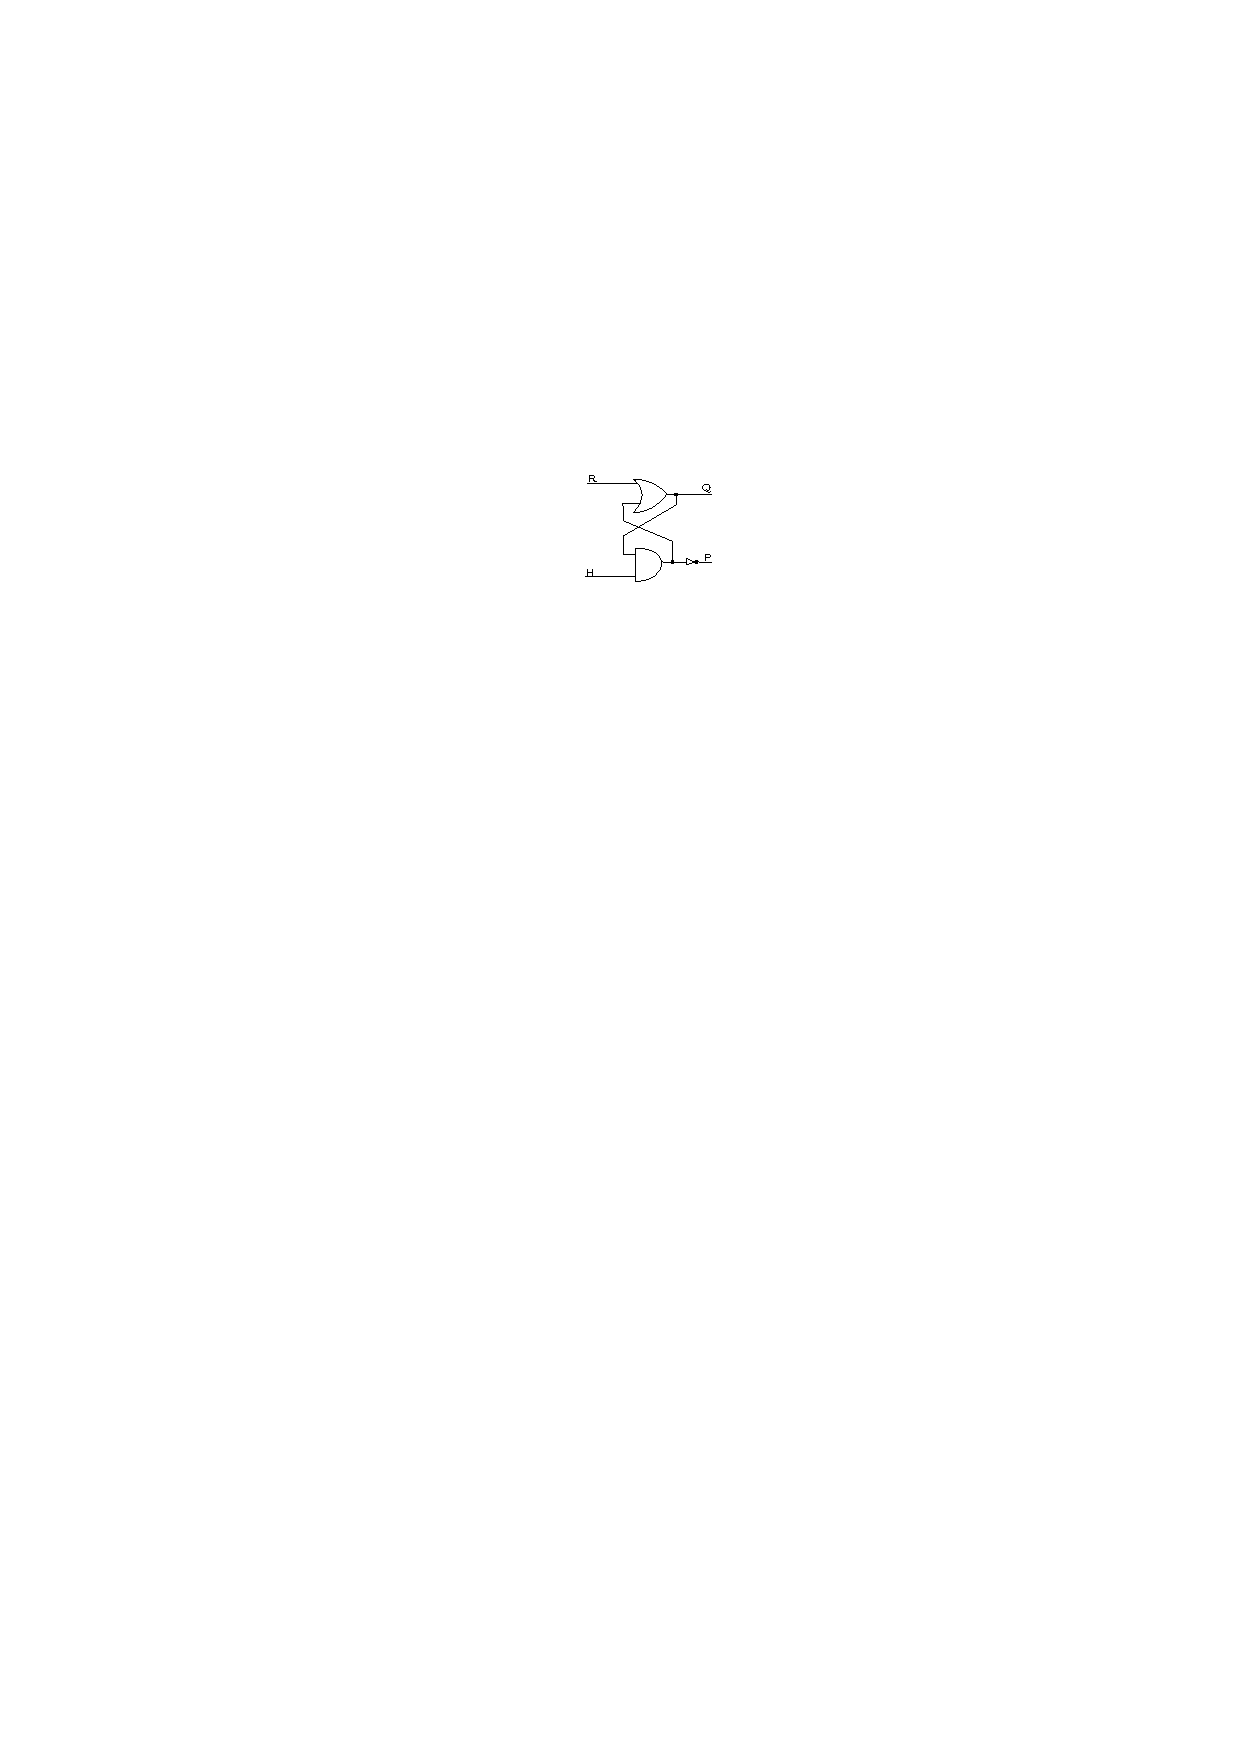
\includegraphics[width=0.3\textwidth]{fig/Q_basic1.pdf}
	\label{fig:Q_basic_1}
\end{figure}